\documentclass[../main.tex]{subfiles}
\begin{document}

The work presented in this Chapter is published in \textcite{Walter_2019}. 

\section{Introduction to the SSD Algorithm}
Stochastic Speckle Discrimination (SSD) is a post-processing technique for direct planet detection designed to reduce the additional noise caused by speckle fluctuations by temporally resolving the intensity variations in the focal plane. It relies on the difference in shape between the on-axis and off-axis intensity distributions \parencite{Soummer_2007a, Gladysz_2008b} or the difference between various moments or combinations thereof \parencite{Gladysz_2009, Gladysz_2010} to enhance the signal of faint companions hidden in stellar light. The first algorithm \parencite{Gladysz_2008} compared the empirical intensity distribution at the location of a suspected companion to a theoretical probability density function (PDF) of a speckle. The difference between distributions was quantified and translated to a confidence level associated with the detection decision. The moment-based approach compared only the parameters of measured distributions \parencite{Gladysz_2009, Gladysz_2010} or their combinations. Expressions involving these parameters are chosen so that stellar light is suppressed while light from a companion is amplified. SSD-like approaches have been shown to reduce speckle noise from even fast atmospheric speckles and improve the contrast limit for the detection of substellar companions \parencite{Frazin_2016, Meeker2018, Stangalini_2018}.

In this Chapter, we present an improved version of SSD to exploit noise-free photon-counting cameras like MEC, the Microwave Kinetic Inductance Detector (MKID) Exoplanet Camera \parencite{Walter2018, Meeker2018} on Subaru Telescope's SCExAO instrument \parencite{Lozi2018}. Our approach statistically distinguishes a combination of constant and speckle intensity (both ultimately from the bright star) from incoherent light (from a planet or disk). At small separations, where ADI and SDI are least effective and the scientific questions are most pressing \parencite{Mawet2012}, we expect SSD to offer strong improvements in the limiting detection contrast. This Chapter describes the new photon counting SSD technique and demonstrates its performance on simulated data. 

We organize the Chapter as follows. In Section \ref{sec:sim} we detail the simulation of photon lists to emulate the data expected from photon-counting cameras like MEC. Section \ref{sec:binned} describes a formal extension of previous SSD analysis techniques with millisecond images using a maximum likelihood algorithm. We simulate the performance for various atmospheric conditions, planet brightnesses, and effective exposure times. Section \ref{sec:binfree} presents the new photon-counting SSD algorithm that estimates the incoherent light from a companion or disk directly from individual photon arrival timestamps. We demonstrate the algorithm on a simulated telescope image. We discuss the main results in Section \ref{sec:discuss}, and conclude with Section \ref{sec:conclusions}. 

\section{Simulating Photon Arrival Times} \label{sec:sim}

\subsection{Modeling the Stellar Speckle Intensity}
The statistics governing the off-axis intensity distribution of coherent light with a partially developed speckle pattern have been studied at length. Originally derived by \textcite{Goodman1975} and verified experimentally by \textcite{Cagigal_2001} and \textcite{fitzgerald_2006}, the probability of getting an instantaneous intensity $I$ given $I_c$ and $I_s$ is governed by the Modified Rician (MR) distribution, defined as:
\begin{equation}
    \rho_{\rm MR}\left[ I | I_c, I_s \right] = \frac{1}{I_s}\exp{\left[ - \frac{I + I_c}{I_s} \right] I_0 \left[ \frac{2 \sqrt{I\,I_c}}{I_s} \right]}, 
    \label{equ:mr}
\end{equation}
where $I_0[x]$ denotes the zero-order modified Bessel function of the first kind. The parameter $I_c$ represents the intensity of the "constant" part of the diffraction pattern, i.e.~the PSF of a star without the atmosphere, while $I_s$ is the intensity of the seeing halo which manifests as a "speckle" pattern \parencite{Canales1999, aime04b, Soummer_2007}.

Typically the AO system attempts to confine all the speckles into the constant diffraction pattern. A coronagraph can remove or transform this coherent portion out of the image plane. For all of the calculations in this Chapter we assume that the Strehl ratio, and by extension $I_c$ and $I_s$, remain constant. 

Speckle intensity is correlated temporally. In the limit of Kolmogorov atmospheric turbulence and frozen flow, the speckle decorrelation time can be thought of as the wind crossing time across the telescope pupil. In reality, the turbulence is not Kolmogorovic, the atmospheric turbulence evolves, and there are often multiple turbulence layers with different wind speeds and directions \parencite{Roddier_1982, Macintosh_2005}. Other high speed processes such as dome seeing, telescope vibrations from wind buffeting, or the AO loop itself can further complicate the speckle temporal power spectrum density (PSD) \parencite{Stangalini_2016}. This may result in a faster speckle decorrelation time, a temporal PSD described by multiple exponential timescales, or possibly a dependence on the position in the focal plane.

For the purposes of creating the simulated data we characterize the speckle PSD as a simple exponential decay with a characteristic speckle lifetime of $\tau_s = 0.1$~s to roughly match empirical data in the near infrared \parencite{fitzgerald_2006, Meeker2018, Goebel_2018}. The speckle lifetime can change drastically depending on the atmospheric conditions but our results here can be qualitatively understood in those cases by scaling all parameters in time. A core condition for the SSD technique is for many photons to arrive in a single speckle decorrelation time: if this is satisfied, individual speckle fluctuations can be probed without relying on prior knowledge of the true speckle temporal PSD.

\subsection{Modeling an Incoherent Source}

For high levels of AO correction that minimize the variations in instantaneous Strehl the light from a companion can be approximated as a delta function with a Poisson intensity distribution \parencite{Gladysz_2008b}. This works well for faint sources where only the core of the PSF is visible. By ignoring variations in the Strehl we simplify our model; incoherent Poisson sources are parameterized by an intensity $I_p$ and can be readily injected into images with the relevant photons uniquely identified in simulation. Any incoherent Poisson sources will be represented by this term including binary companions, planetary companions, extended sources, dark current, and read noise. For the coherent stellar light, in the case that $I_s=0$, the MR distribution reduces to a Poisson distribution with intensity $I_c$ and will be indistinguishable from $I_p$. In the demonstrations that follow, we identify $I_p$ as an injected planetary companion. 

The intensity fluctuations associated with speckles elevate the noise floor above the typical shot noise, i.e., it is harder to measure the planet's intensity when it is embedded in a boiling speckle field. If the speckle temporal information is marginalized over, then we show in Appendix \ref{appendix:a} that the total variance of temporally correlated intensities obeying MR statistics combined with photon shot noise is 
\begin{equation}
    \sigma^2_{I, \rm tot} \approx \frac{2\tau_s \left( I_s^2 + 2 I_c I_s \right) + I_c + I_s + I_p}{T_{\rm tot}}.
    \label{eq:totalnoise}
\end{equation}
The variance of the measured intensity is inversely proportional to the total integration time, $T_{tot}$, as expected. This is the long exposure ($t_\mathrm{exp} \gg \tau_s$) photon noise limit faced by all PSF subtraction techniques like ADI and SDI. In the limit that $2\tau_s I_s \ll 1$, this variance reduces to pure shot noise on the number of photons. For high contrast imaging, typical parameters might be $\tau_s=0.1$~s, $I_s=50$~s$^{-1}$, and $2\tau_s I_s = 10$, in which case the noise from speckle fluctuations will dominate. In Section \ref{sec:binfree}, we show that this noise can be overcome by temporally resolving individual fluctuations in the speckle background. 

\subsection{Generating Mock Photon Lists}

We have developed code\footnote{Part of MKID Pipeline python package available at https://github.com/MazinLab/MKIDPipeline} for quickly generating mock photon lists with an optional injected planet, corresponding to the output of a single MKID-like pixel which is single photon counting with low noise. The photon lists obey the following rules: 

\begin{enumerate}
    \item The underlying intensities are MR distributed, but are correlated in time with $\langle I(t)I(t + \delta t )  - \langle I \rangle^2 \rangle \propto \exp{\left[-\delta t / \tau_s\right]}$. 
    \item $I_c$, $I_s$, and $I_p$ are independently specified by the user, such that $I_c$ and $I_s$ govern the MR statistics of the stellar intensity and $I_p$ is the mean count rate of a Poisson source. The total intensity should have an expectation value of $\left\langle I \right\rangle = I_c + I_s + I_p$. 
    \item Due to the intrinsic dead time in an MKID, photons are removed from the list if they arrive within $\tau_0$ of the previous valid photon's arrival time. 
\end{enumerate}

The procedure for generating photon timestamps begins with creating a correlated list of random numbers that follow a Gaussian distribution. The random numbers are transformed to a uniform distribution ranging from 0 to 1, and finally transformed again to a MR distribution. The correlated MR sequence defines the intensity in photon counts for a small ($\ll \tau_s$) time bin (we used 200~$\mu$s), and a Poisson draw on that ``instantaneous'' intensity determines the number of photons that will finally be placed into that bin. The photons are distributed according to a uniform distribution in each bin. For simplicity, we assume neighboring pixels to have uncorrelated photon lists. 

Since MKIDs do not have the same dark current or readout noise as conventional semiconductor detectors we do not add any additional noise. However, during high count rates photons can be lost due to a firmware triggering lockout that acts as a non-paralyzable dead time \parencite{Eyken_2015}. We use $\tau_0 = 10~\mu$s to match the latest firmware implemented on MEC. This dead time formulation could be used with quasi-photon counting EMCCDs to account for photon pile-up. 

\section{SSD with Short Exposure Images} \label{sec:binned}

Past efforts have been successful in detecting the position of (real or synthetic) faint companions in high contrast images. \textcite{Gladysz_2008} and \textcite{Meeker2018} fit histograms of light curves (see top/middle of Figure \ref{fig:SSD_bin}) and discriminate planets by extracting parameters of hypothesized distributions using e.g. the method of moments and comparing those parameters, or their combinations, to the rest of the field. For example, a large $I_c/I_s$ ratio can be used as a merit function since faint companions can masquerade as static speckles. \textcite{Stangalini_2018} use a discriminator from a direct recurrence quantification analysis of the light curves to search for companions. \textcite{Gladysz_2009, Gladysz_2010} also fit histograms of the light curves but use a deconvolution of the modeled probability distribution functions to further extract the companion's photometry.

In this section we extend previous work by  extracting the position and photometry of astrophysical sources (point or extended sources) using a maximum likelihood algorithm.

\begin{figure}
    \centering
    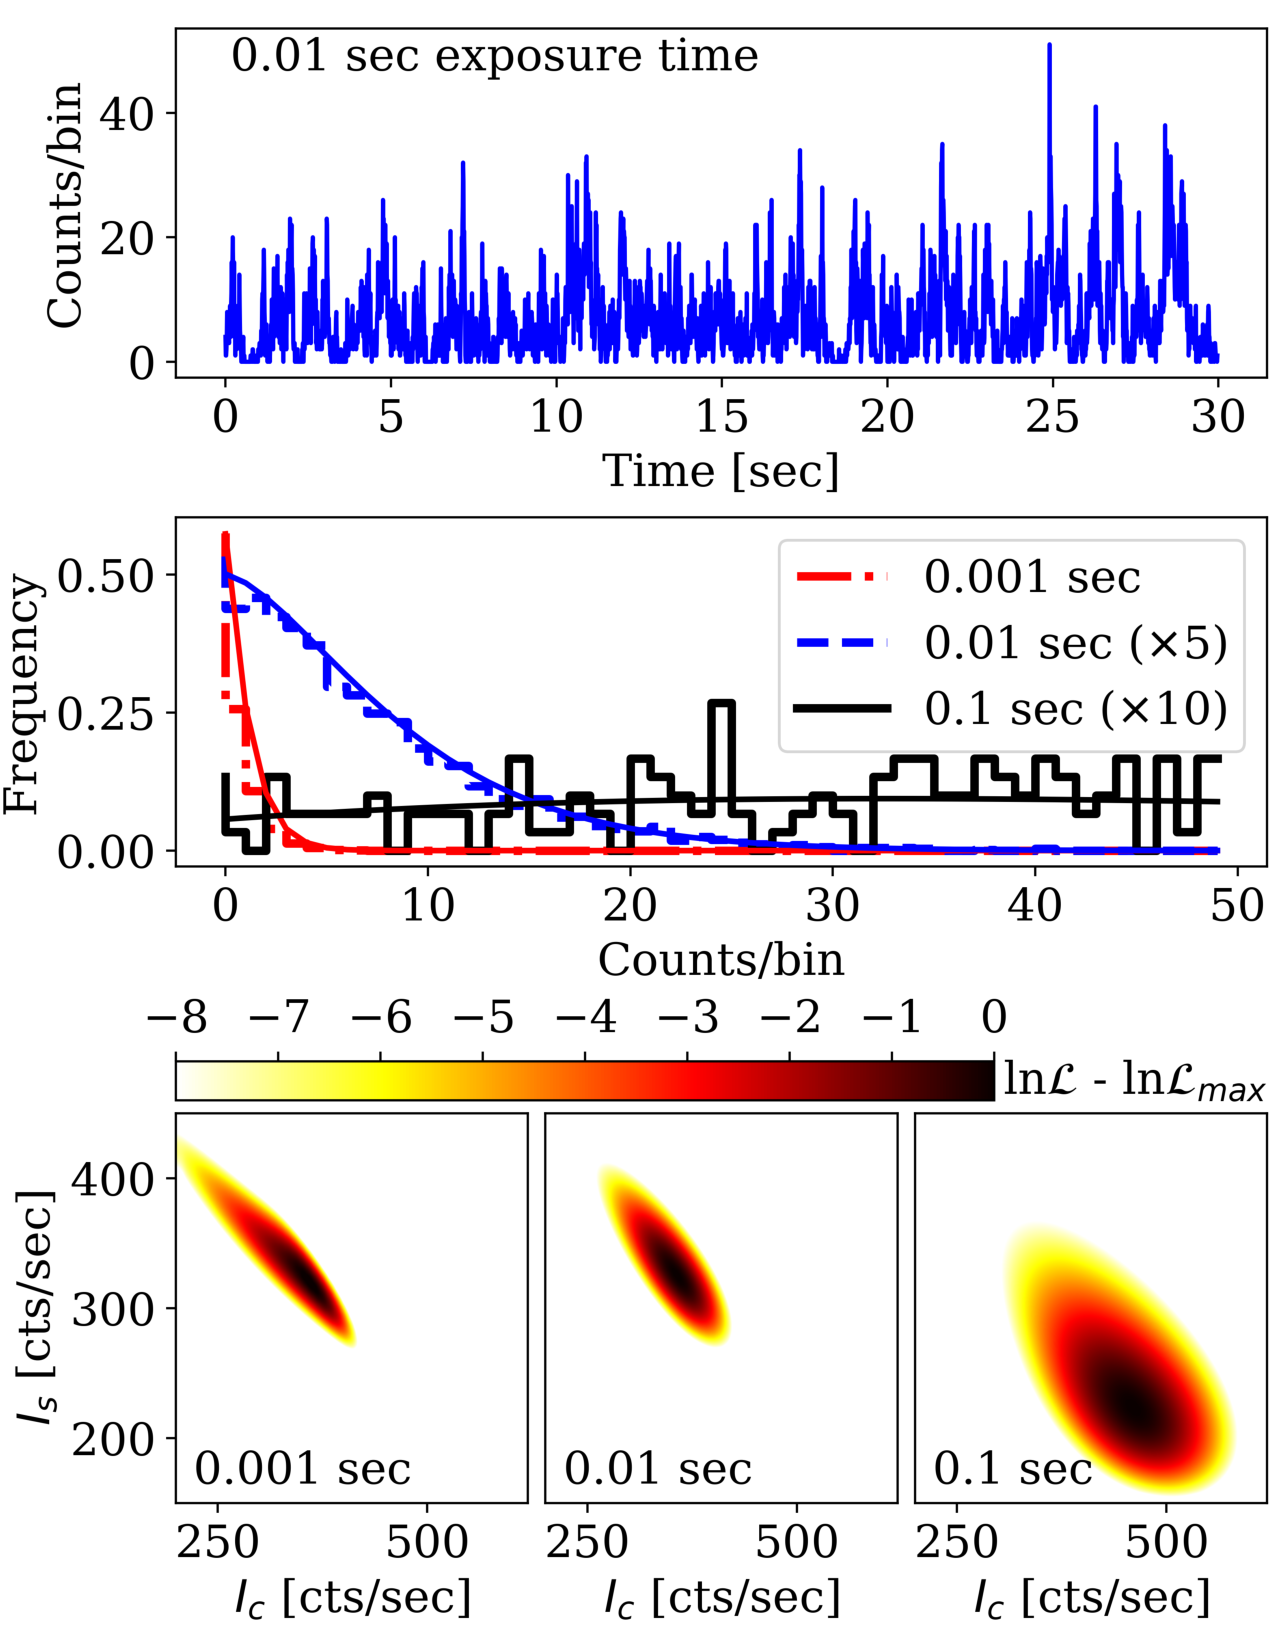
\includegraphics[width=0.6\textwidth]{binned.pdf}
    \caption[Simulating lightcurves and calculating the most likely $I_c$ and $I_s$]{Top: a 30~s mock photon list simulated using the parameters $I_c = 300$, $I_s = 300$, $I_p = 0$ photons/s with $\tau_s=0.1$~s, is binned into 0.01~s exposures to form a light curve. Middle: The same photon list is binned by three different exposure times and used to plot intensity histograms. The best-fit modified Rician functions are overplotted. The distribution changes shape as the bin size is varied; the corresponding fitted parameters also change. The histograms for 0.01 and 0.1~s exposure times have been scaled by factors of 5 and 10 respectively. Bottom: the likelihood is marginalized over $I_p$ for the three different exposure times to illustrate how the best fit parameters evolve with bin size. The darkest area in the plot represents the maximum likelihood and determines the best fit values of $I_c$ and $I_s$. The same photon list was used for all plots. }
    \label{fig:SSD_bin}
\end{figure}

\subsection{Maximum Likelihood Model for Discrete Light Curves}

We model the intensity in the focal plane with three parameters $I_c$, $I_s$, and $I_p$ and calculate their most likely values with an algorithm operating on the light curve. This allows for a direct detection of the non-stellar intensity, $I_p$, in the form of a point source like a planet or an extended source like a protoplanetary disk. Furthermore, we can naturally introduce photon noise from a low-intensity photon counting regime. By allowing the MR distribution in Equation \eqref{equ:mr} to suffer a Poisson-Mandel transformation \parencite{cagigal_1999, aime04b}, the discrete stellar intensity distribution becomes
\begin{align}
p_\star [ n| I_c,I_s] &=\int_{0}^{\infty} \frac{I^n}{n!}\exp\left[-I\right]\rho_{\rm MR}[I]dI \nonumber\\
&= \frac{1}{I_s + 1}\left( 1 + \frac{1}{I_s} \right)^{-n} \exp\left[ -\frac{I_c}{I_s} \right] \nonumber \\ & \quad \times L_n\left[ \frac{-I_c}{I_s^2 + I_s} \right] \exp\left[  \frac{I_c}{I_s^2 + I_s}  \right],
\end{align}
where $L_n$ is the $n^{\mathrm{th}}$ Laguerre polynomial. The units of intensity for this section are number of photons per exposure time, $t_\mathrm{exp}$. If a planet (or some other source that is incoherent with the star) exists in the field, the intensity distribution at that location will be the discrete convolution of $p_\star$ with the planet's independent probability distribution $p_p$. To simplify, we assume the incoherent source has a Poisson probability distribution, $p_p [m | I_p] = \exp\left[ -I_p \right] I_p^m/m! $ with average intensity $I_p$. The likelihood of the $i$th bin of a light curve containing $k$ photons given $I_c$, $I_s$, and $I_p$ is 
\begin{equation}
\mathcal{L}_i = \sum_{m=0}^{k_i} p_p[m|I_p]p_\star[k_i-m|I_c,I_s],
\end{equation}
which becomes
\begin{align}
\label{equ:binnedLogL}
\mathcal{L}_i  =  &\frac{1}{I_s + 1} \exp\left[ -I_p -\frac{I_c I_s}{I_s^2 + I_s}  \right] \nonumber \\ &\times \sum_{m=0}^{k_i}  \frac{I_p^m}{m!} \left( 1 + \frac{1}{I_s} \right)^{-(k_i-m)} \ L_{k_i-m}\left[ \frac{-I_c}{I_s^2 + I_s} \right].
\end{align}
The likelihood of the entire light curve is $ \mathcal{L} = \prod_i \mathcal{L}_i$. We use a L-BFGS-B optimizer to find the most likely values of $I_c$, $I_s$, and $I_p$. 

The maximum likelihood estimate of the intensity distribution is overplotted onto the light curve histograms for three different exposure times in the middle panel of Figure \ref{fig:SSD_bin}. The bottom panel shows the likelihood functions marginalized over $I_p$ for these three exposure times. 

\subsection{Performance of Millisecond Imaging SSD}

To understand the performance of this millisecond imaging SSD algorithm and the extent to which it can improve exoplanet detections, we produce receiver operator characteristic (ROC) curves \parencite{Tanner1954,DeLong+DeLong+Clarke-Pearson_1988,Krzanowski2009,Jensen_Clem_2017}. We achieve this by generating an ensemble of mock photon lists with the same nominal values of $I_c$, $I_s$, and $I_p=0$ and calculating maximum likelihood estimates to build up a distribution of $I_p$ corresponding to the signal-absent hypothesis. Next we inject a planet with $I_p>0$ and calculate maximum likelihood estimates to build a distribution for $I_p$ corresponding to the signal-present hypothesis. These distributions are shown in the left column of Figure \ref{fig:rocVsBin}. By choosing a detection threshold, we can calculate a true positive rate and false positive rate from the signal-present distribution and signal-absent distribution respectively. The ROC curves in the right column of Figure \ref{fig:rocVsBin} are generated by varying the detection thresholds.

The right column of Figure \ref{fig:rocVsBin} demonstrates the performance of the millisecond imaging SSD algorithm for different exposure times. The shape of the discrete intensity distribution can change depending on exposure time, which systematically affects the resulting maximum likelihood estimates (MLE) for $I_c$, $I_s$, and $I_p$ along with their uncertainties. In some cases there is a significant probability for the most likely value of $I_p$ to be equal to zero. In the case that $I_c \gg I_s$, the MLE probability can be multimodal with a significant peak at $\textrm{MLE}~I_p \approx \textrm{True}~I_c + \textrm{True}~I_p$. Both these behaviors appear for the same reason: when there is little modulation by $I_s$ of photons associated with $I_c$, then $I_c$ becomes difficult to distinguish from $I_p$. However, the total flux is still accurately recovered. 

\begin{figure*}
    \centering
    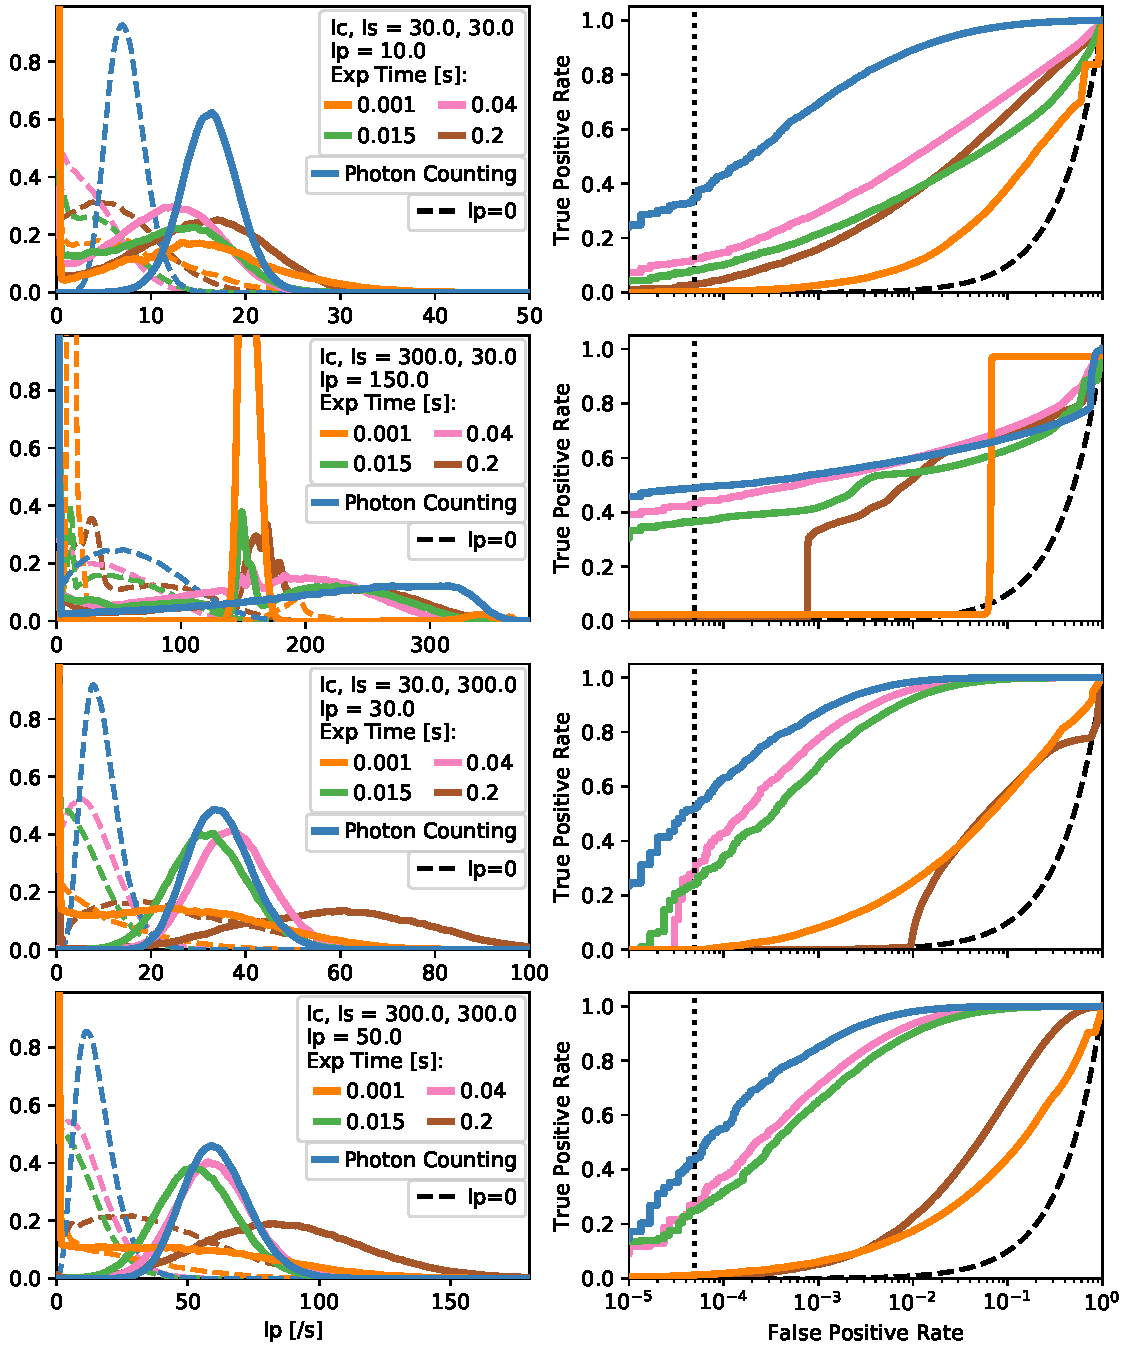
\includegraphics[width=0.85\textwidth]{rocVsBin.pdf}
\caption[ROC curve performance of the millisecond imaging SSD algorithm]{Performance of our millisecond imaging SSD algorithm (Section \ref{sec:binned}) compared to our photon counting SSD algorithm (Section \ref{sec:binfree}). Left panels: histograms of the maximum likelihood estimates of $I_p$, computed using $3\cdot 10^5$ 30~s mock photon lists. Maximum likelihood estimates for $I_p$ are calculated for various effective exposure times and for the case with (solid line) and without ($I_p=0$, dashed line) an injected planet. The $y$-axis in the left column is arbitrary. The probability distributions are used to calculate the true/false positive rates for the receiver operator characteristic (ROC) curve (right). The vertical dotted line at 1/20000 (for the 20000 pixels in MEC) roughly indicates the maximum tolerable false positive rate. The full photon-counting SSD algorithm (blue lines) described in Section \ref{sec:binfree} outperforms the cases with nonzero exposure times.}
    \label{fig:rocVsBin}
\end{figure*}

We find that there exists an optimal camera frame rate that leads to the most precise probability distribution for $I_c$, $I_s$, and $I_p$. For exposure times that are too short ($t_\mathrm{exp} \ll \delta t$, the photon inter-arrival time) the correlation between subsequent photon arrivals is lost because frames are interpreted as an unordered set containing only 0 or 1 photons. For exposure times that are too long ($t_\mathrm{exp} \gg \tau_s$) the speckle temporal information is averaged over. This tends to artificially decrease the $I_s$ component of the speckle intensity directly in exchange for increasing the $I_c$ component (see Fig \ref{fig:SSD_bin} bottom). For those that use $I_c / I_s$ as a merit function this means the part of the image without a planet will be polluted making it harder to discriminate the location of a companion.





\section{SSD in the Photon Counting Regime} \label{sec:binfree}

\subsection{Maximum Likelihood Model for Photon Arrival Times}

In the previous section the most precise extraction of the model parameters $I_c$, $I_s$, and $I_p$ required the use of an optimal exposure time. Since this optimal exposure time is dependent on the speckle intensity as well as the speckle decorrelation time, the optimal exposure time will vary across the image. Conversely, if a single exposure time is chosen there may be a systematic loss of precision across some portions of the image. In order to avoid this pitfall, we develop the posterior probability for $I_c$, $I_s$, and $I_p$ directly from the set of photon inter-arrival times. 

We start by considering the (normalized) probability density for the next inter-photon arrival interval, $\delta t$, given a fixed intensity $I$:
\begin{equation}
\begin{aligned}
p[\delta t | I] = I e^{-I \delta t}.
\label{equ:poisson}
\end{aligned}
\end{equation}
The speckle field intensity is not fixed but varies in time with the modified Rician probability density described in Equation \eqref{equ:mr}. At a fixed point in time, the probability density of the next photon arrival time given $I_c$ and $I_s$ becomes
\begin{equation}
\begin{aligned}
p[\delta t | I_c, I_s] = \int_{0}^{\infty} p[\delta t | I] \rho_{\rm MR} [I | I_c, I_s] dI,
\end{aligned}
\end{equation}
where we have integrated the Poisson probability density from Equation \eqref{equ:poisson} over all possible instantaneous stellar intensities, $I$. Intensities are considered to be in units of photons per second. We assume here that the speckle lifetime is much longer than the time it takes a photon to arrive, $\tau_s \gg \delta t$. 

With a set of photon inter-arrival times, $\{\delta t_{i}\}$, we want the relative probability that a $\delta t$ is realized. At moments that happen to have higher instantaneous intensities the number of short $\delta t_{i}$'s will be increased. Thus, the relative probability of a photon inter-arrival time being in our data becomes
\begin{equation}
\begin{aligned}
p[\delta t | I_c, I_s] \propto \int_{0}^{\infty} p[\delta t | I] \rho_{\rm MR} [I | I_c, I_s] I dI.
\end{aligned}
\end{equation}
Finally, we consider the case that light incoherent with the star, such as from a planet, is in the field. We consider only the simplest case in which this source has constant intensity $I_p$ and is governed by Poisson statistics. In this case, the relative probability of $\delta t$ given $I_c$, $I_s$, $I_p$ is
\begin{equation}
\begin{aligned}
p[\delta t | I_c, I_s, I_p] \propto \int_{0}^{\infty} p[\delta t | I + I_p] \rho_{\rm MR} [I | I_c, I_s] (I + I_p) dI,
\label{eq:mr_deltat_like}
\end{aligned}
\end{equation}
which can be evaluated analytically. We then find the normalization constant by setting
\begin{equation}
\begin{aligned}
\int_{\tau_{0}}^{\infty} p[\tau | I_c, I_s, I_p] d\tau = 1.
\end{aligned}
\label{eq:normalization}
\end{equation}
Equation \eqref{eq:normalization} accounts for the non-paralyzable detector dead time, $\tau_0$, intrinsic to MKIDs by replacing the lower limit of integration with $\tau_0$. In Equation \eqref{eq:mr_deltat_like}, we set the likelihood equal to zero for $\delta t < \tau_0$. It is convenient to use the change of variables,
\begin{equation}
\begin{aligned}
u_i=\frac{1}{1+I_s \delta t_i}~,~~u_{max}=\frac{1}{1+I_s \tau_0}.
\end{aligned}
\end{equation}
The log-likelihood, $\log(\mathcal{L})[I_c, I_s, I_p]$, then becomes
\begin{align}\label{equ:binfreeLogL}
    \log(\mathcal{L})=& \sum_{i=1}^{N} p[\delta t_i | I_c, I_s, I_p] \nonumber\\
    =&\sum_{i=1}^{N}(u_i - 1) \left(\frac{I_p}{I_s u_i}+\frac{I_c}{I_s} \right)  \nonumber\\
    &+\sum_{i=1}^{N} \log\big[I_c^2 u_i^5 + 4 I_c I_s u_i^4 + (2 I_s^2 + 2 I_p I_c)u_i^3 \nonumber\\[-10pt]
    &~~~~~~~~~~~~~+ 2 I_p I_s u_i^2 + I_p^2 u_i\big]  \nonumber\\[3pt]
    &-N \frac{(u_{max}-1)(I_p + I_c u_{max})}{I_s u_{max}}  \nonumber\\[2pt]
    &-N \log\left[I_c u_{max}^3 + I_s u_{max}^2 + I_p u_{max}\right] .
\end{align}
As in Section \ref{sec:binned}, we assume that AO performance remains stable so that $I_c$ and $I_s$ remain constant over the course of observations. 

Equation \eqref{equ:binfreeLogL} for the photon counting SSD algorithm replaces Equation \eqref{equ:binnedLogL} from Section \ref{sec:binned}. We use a Newton conjugate-gradient search to find the maximum of the log-likelihood space and recover the best estimates for $I_c$, $I_s$, and $I_p$. 

The photon-counting SSD algorithm consistently outperforms the millisecond imaging SSD algorithm from Section \ref{sec:binned}, which marginalizes over temporal information via the exposure time (see Figure \ref{fig:rocVsBin}). In Figure \ref{fig:rocVsIp} we show the performance of the photon counting SSD algorithm under conditions given by various combinations of $I_c$ and $I_s$, and with various planet brightnesses $I_p$. The algorithm performs well with a high true positive detection rate even for the case when $I_c$ and $I_s$ are both large. However, the performance suffers in the case of $I_c \gg I_s$. As in millisecond imaging SSD, $I_p$ and $I_c$ become indistinguishable in this limit. 

\begin{figure*}
    \centering
    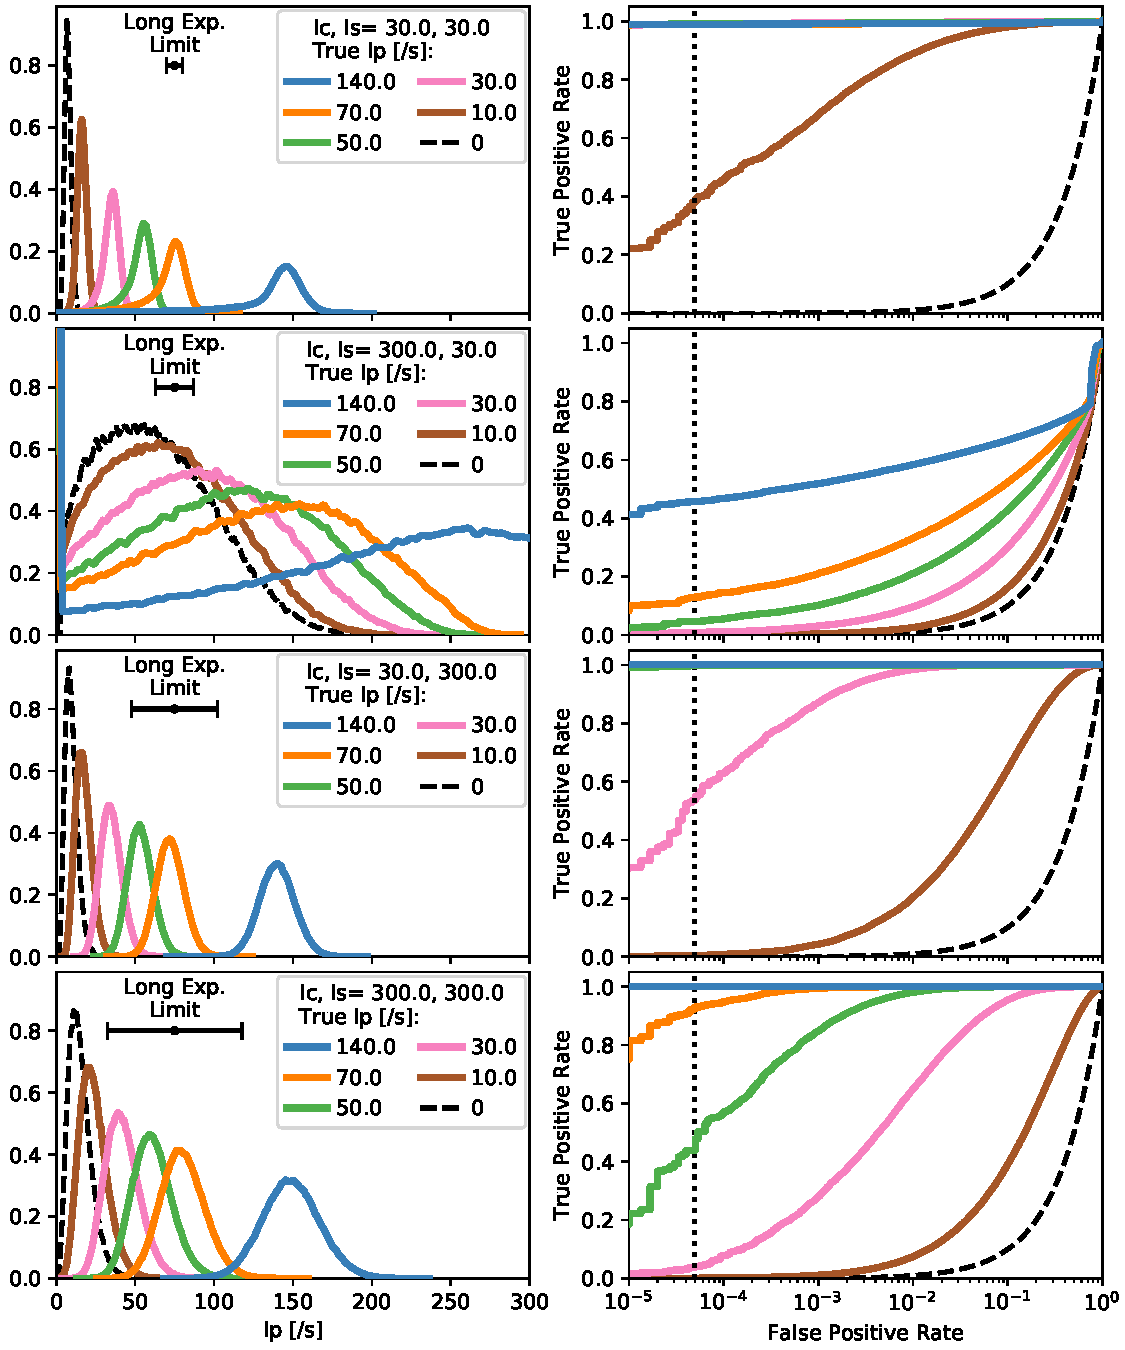
\includegraphics[width=0.85\textwidth]{rocVsIp.pdf}
    \caption[ROC curve performance of the photon-counting SSD algorithm]{Performance of our photon-counting SSD algorithm. Left panels: histograms of the maximum likelihood estimates of $I_p$, computed using $3\cdot 10^5$ 30~s mock photon lists for each set of parameters. The $\pm\sigma$ for the long exposure photon noise limit (Equation \eqref{eq:totalnoise}) is shown with an error bar. The $y$-axis in the left column is arbitrary. The probability distributions are used to calculate the true/false positive rates for the receiver operator characteristic (ROC) curve (right panels). The vertical dotted line at 1/20000 (for the 20000 pixels in MEC) roughly indicates the maximum tolerable false positive rate. The algorithm performs well with a high true positive detection rate even for the case when $I_c$, $I_s$ are both large. However, the performance suffers in the case of $I_c \gg I_s$ (row 2). }
    \label{fig:rocVsIp}
\end{figure*}

\subsection{Maximum A Posteriori Estimation}

Prior knowledge of a parameter can improve the estimates of $I_c$, $I_s$, and $I_p$. In our case, we commonly have information on the $I_c$ parameter which corresponds to the static or quasi-static speckle point spread function either from a telescope model or measured on a reference star. For such situations, the log likelihood function in Equation \eqref{equ:binfreeLogL} can be modified with a Gaussian prior as
\begin{equation}
\begin{aligned}
\log(\mathcal{L}) \rightarrow \log(\mathcal{L}) - \frac{1}{2} \left(\left(I_c - \tilde{I}_c\right)/\sigma[\tilde{I}_c]\right)^2
\end{aligned}
\end{equation}
where $\tilde{I}_c \pm \sigma [\tilde{I}_c]$ is the prior on $I_c$. The new estimates of $I_c$, $I_s$, and $I_p$ become maximum a posteriori (MAP) estimates. 

\subsection{Performance on Simulated Telescope Image}

\begin{figure*}
    \centering
    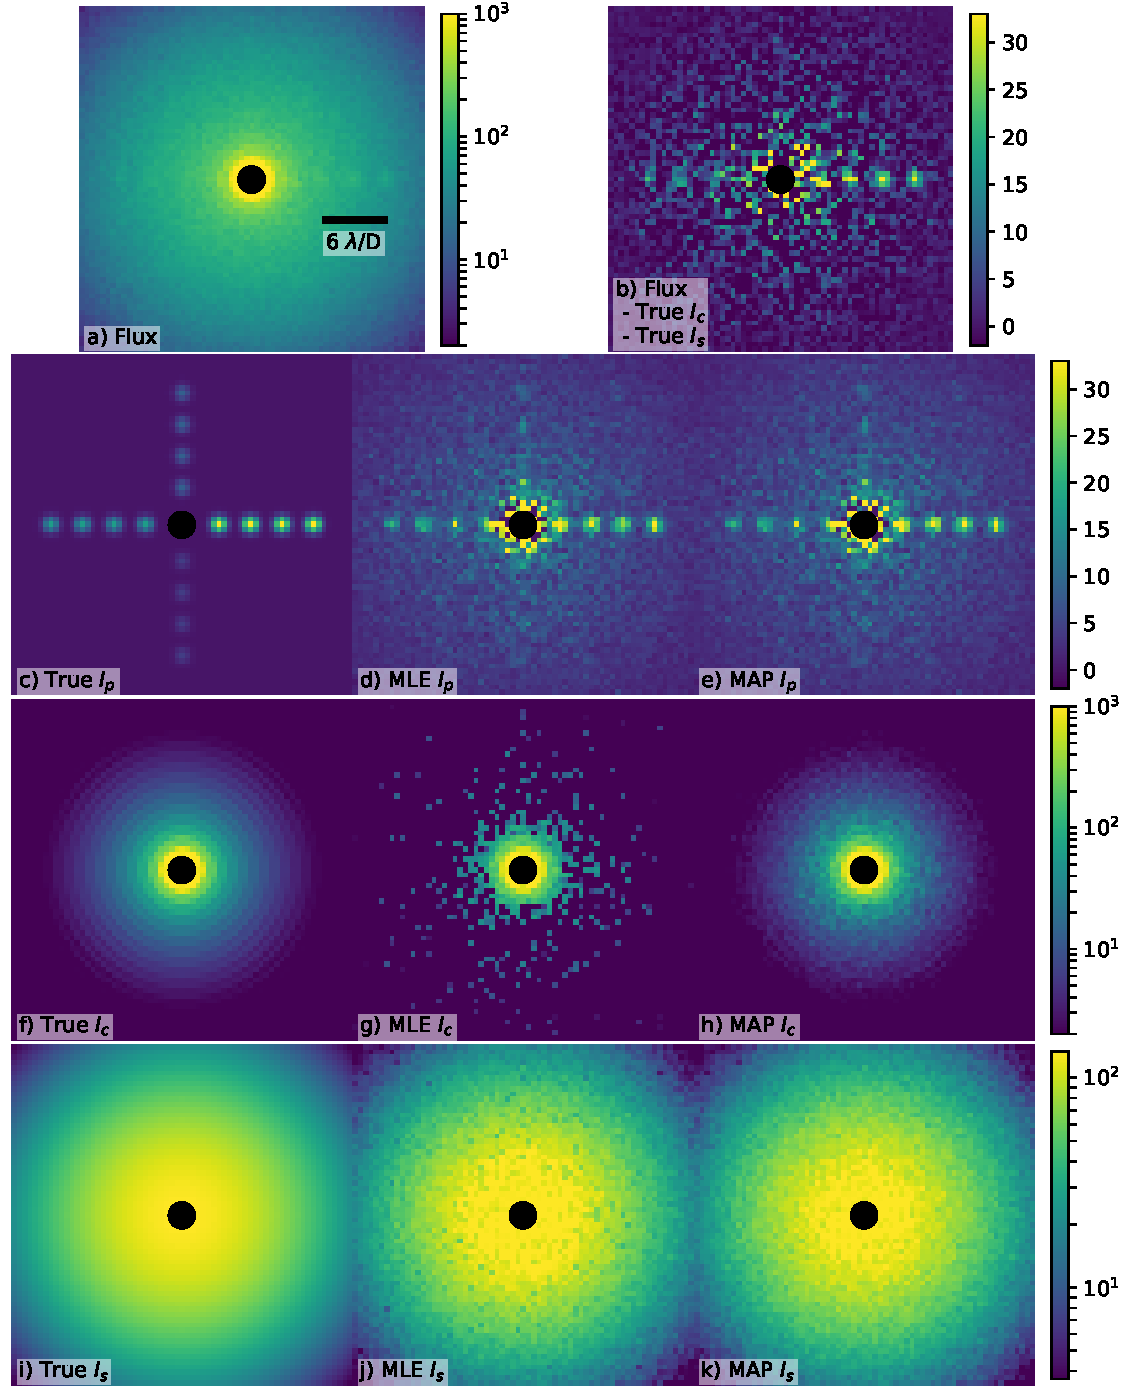
\includegraphics[width=0.75\textwidth]{simSSD.pdf}
    \caption[The photon-counting SSD algorithm using simulated telescope images]{Performance of our photon-counting SSD algorithm on simulated telescope images.  Panel (a) shows the average intensity of simulated photon lists in each pixel; panels (c), (f), and (i) show the parameters used. Panel (b) subtracts stellar flux from (f) and (i) from the average intensity, (a), illustrating the speckle variance in a long exposure image. Panel (b) represents the theoretical limit of perfect PSF subtraction in a single exposure subject to MR intensity fluctuations. The photon-counting SSD algorithm results in the maximum likelihood estimates shown in (d), (g), and (j). Using a priori knowledge of the $I_c$ parameter (we used a Gaussian prior of True $I_c \pm 3\cdot \sqrt{\text{True}~I_c}$) we generate the maximum a posteriori (MAP) estimates shown in (e), (h), and (k). The planet signals extracted from the MAP $I_p$ estimate in (e) are not significantly improved compared to the MLE $I_p$ in (d). However, the SSD results in (d) and (e) both extract the planet better than the perfect PSF subtraction shown in (b). All images represent 30~seconds of data on a magnitude $J=10$ star with an 8.2~m telescope; all units are photons/second. 
    }
    \label{fig:image}
\end{figure*}

We evaluate the performance of the photon-counting SSD algorithm on a simulated 30~s telescope image without a coronagraph. We identify $I_c$ as the Airy-ring pattern of a diffraction limited telescope with a circular unobstructed aperture, $I_s$ as the seeing halo from atmospheric speckles with a Strehl ratio of 0.7, and $I_p$ as a series of injected planets at various brightnesses and separations. The faintest planet's total intensity is 40~photons/s, for a contrast of $5 \cdot 10^{-5}$ with the host star, and is separated by 3.5~$\lambda$/D. Assuming a 5\% end-to-end throughput on an 8.2~m telescope, the stellar magnitude in the near infrared is approximately $J=10$. We assume a speckle decorrelation time of $\tau_s=0.1$~s and detector dead time of $\tau_0=10$~$\mu$s.

Each pixel has an independent 30~s photon list generated from the ``True'' $I_c$, $I_s$, and $I_p$ shown in panels (c), (f), and (i) respectively of Figure \ref{fig:image}. Spatial correlations in the photon lists are ignored for simplicity. The average intensity realized for each pixel is shown in Figure \ref{fig:image}a. Figure \ref{fig:image}b is the average intensity minus the expected light from the star, $(\textrm{True}~I_c + \textrm{True}~I_s)$, which illustrates the best possible long exposure PSF subtraction (compare the background variance to Equation \eqref{eq:totalnoise}). The MLE $I_c$, $I_s$, and $I_p$ are shown in Figure \ref{fig:image}d, g, and j respectively. In Figure \ref{fig:image}e, h, and k, we calculate the MAP estimates. We used the True $I_c \pm 3\cdot \sqrt{\text{True}~I_c}$ as a Gaussian prior on $I_c$; in practice one could use a telescope model or a reference PSF. The central black dot with radius 1.22~$\lambda$/D is not a coronagraph but simply obscures the on-axis light for convenience. 

Comparing Figure \ref{fig:image}d to Figure \ref{fig:image}b shows that the MLE $I_p$ from the photon counting SSD algorithm recovers the injected planets better than a perfect stellar PSF subtraction (i.e.~subtraction of the true $I_c$ and $I_s$). Figure \ref{fig:image}d and e show that the MAP estimate for $I_p$ is not significantly better than the MLE $I_p$ (although the MAP estimate for $I_c$ is more precise). This is surprising because the MAP estimate includes a prior on $I_c$ that should help discriminate between $I_c$ and $I_p$. That this is not the case indicates we can take full advantage of the photon counting SSD algorithm without prior knowledge of the telescope PSF. 

For the central pixel of each planet, we used $10^5$ independent photon lists to calculate the signal-to-noise ratio $\textrm{S/N}=(\langle I_p \rangle - \langle \textrm{Background}\rangle) / (\textrm{std. dev.} \langle I_p \rangle)$ where the $\langle \textrm{Background}\rangle$ is estimated by not injecting a planet. These are recorded in Table \ref{tab:mleSN}. The long exposure photon noise limit is also recorded in Table \ref{tab:mleSN} where the estimated $I_p$ is equal to the total flux minus the light from the star, $(\textrm{True}~I_c + \textrm{True}~I_s)$. While the results are from the simulated ensemble, they match the results from Equation \eqref{eq:totalnoise}. Table \ref{tab:mleSN} is representative of 30~seconds of data, but the S/N will scale with $\sqrt{T_{\rm tot}}$. For a 2 minute exposure, all values in Table \ref{tab:mleSN} should be scaled up by a factor of 2. The S/N was calculated using only the central pixel for convenience but would be larger if the surrounding pixels were considered.

\begin{table}[!t]
  \footnotesize
  \setlength{\tabcolsep}{1pt}
  \centering
  \caption{Companion SSD Signal-to-Noise Ratio}
  \label{tab:mleSN}
  \begin{tabular}{l@{\hspace{5pt}}c@{\hspace{5pt}}c@{\hspace{10pt}}ccc@{\hspace{5pt}}c@{\hspace{10pt}}ccc@{\hspace{5pt}}c@{\hspace{10pt}}ccc@{\hspace{5pt}}c@{\hspace{10pt}}cr}
  \hline\hline
  & & \multicolumn{3}{c}{${\rm Separation} = 3.5\,\lambda/D$}
  & & \multicolumn{3}{c}{${\rm Separation} = 6.5\,\lambda/D$}
  & & \multicolumn{3}{c}{${\rm Separation} = 9.5\,\lambda/D$}
  & & \multicolumn{3}{c}{${\rm Separation} = 12.5\,\lambda/D$} \\
  
  Contrast & & MLE & MAP & Limit$^{\rm a}$ 
  & & MLE & MAP & Limit$^{\rm a}$ 
  & & MLE & MAP & Limit$^{\rm a}$
  & & MLE & MAP & Limit$^{\rm a}$\\
  \hline
  
  $4 \cdot 10^{-4}$ && 4.8 & 5.3 & 2.3 && 6.8 & 7.0 & 3.8 && 7.6 & 8.3 & 5.7 && 7.0 & 9.4 & 8.8 \\
  $2 \cdot 10^{-4}$ && 2.8 & 3.0 & 1.2 && 4.0 & 4.0 & 1.9 && 4.9 & 4.9 & 2.9 && 5.6 & 5.9 & 4.5 \\
  $1 \cdot 10^{-4}$ && 1.6 & 1.7 & 0.6 && 2.3 & 2.3 & 1.0 && 2.8 & 2.8 & 1.4 && 3.5 & 3.5 & 2.3 \\
  $5 \cdot 10^{-5}$ && 0.9 & 0.9 & 0.3 && 1.3 & 1.2 & 0.5 && 1.6 & 1.5 & 0.7 && 2.0 & 2.0 & 1.1 \\
  \hline

  \end{tabular}\\
  \begin{itemize}
  \item[] $^{\rm a}$Detection limit for a 30~s long exposure with perfect PSF subtraction of the stellar light.
  \end{itemize}
\end{table}


\section{Discussion of SSD Simulations} \label{sec:discuss}

While it remains impossible to beat the photon shot noise $\sqrt{N}$, Figure \ref{fig:image} shows that the photon counting SSD algorithm can beat the long exposure ($t_\mathrm{exp} \gg \tau_s$) photon noise limit described by Equation \eqref{eq:totalnoise}. Table \ref{tab:mleSN} quantifies the improvement in the S/N as a factor of 3 in the case of faintest planet ($5\cdot 10^{-5}$) at the nearest separation ($3.5~\lambda/D$). This is possible because the speckle fluctuations are temporally resolved ($t_\mathrm{exp} \ll \tau_s$) and individual speckles are probed by multiple photons ($\delta t \ll \tau_s$). In the case that the fluctuations from stellar speckles dominate the variance of the total intensity ($2 I_s \tau_s \gg 1$), fast, noiseless detectors like MKIDs or EMCCDs are needed to dig beneath the noise. This can occur in high contrast imaging at separations between $1~\lambda/D > r <$ seeing radius but is especially important at $\lesssim 5~\lambda/D$ where ADI and SDI start to lose their effectiveness (depending on spectral coverage, sky rotation, and AO performance).

SSD will benefit ADI and SDI by reducing speckle noise from the data that is fed into those algorithms. ADI processing can be approached the same way as usual, but instead of using raw images one would use the $I_p$ images produced with SSD. The modulation of the planet location will be unaffected by SSD. Similarly for SDI, the algorithm would be given $I_p$ maps at various wavelengths. This approach would require wavelength information for each detected photon, which is an intrinsic feature of an MKID detector. 

Our SSD algorithm does not perform well when $I_c \gg I_s$ as seen in Figure \ref{fig:rocVsIp}. In this regime there is little modulation of the static speckle intensity $I_c$ by the atmospheric speckle field $I_s$, and as a result $I_c$ starts to become indistinguishable from the Poisson distributed $I_p$. This can be greatly mitigated with a coronagraph and possibly active speckle nulling \parencite{Martinache_2014} which directly reduce $I_c$ in the image. 

On a space-borne telescope atmospheric speckles are not a concern, implying that the image-plane intensity will have different temporal behavior from ground-based observatories. While our SSD algorithm relies on the intensity following a MR distribution, in general any distribution can be used so long as it is known. It may also be possible to modulate speckles in a controlled way using onboard AO. 


\section{SSD Algorithm Conclusions and Future Work} \label{sec:conclusions}

We can exploit photon arrival time statistics with a stochastic speckle discrimination (SSD) algorithm to distinguish planets from speckles. We first extend previous work with a formalized maximum likelihood algorithm operating on light curves with fixed, albeit fast, exposure times. We find that the likelihood space can sometimes result in bimodal behavior in the case of $I_c \gg I_s$. Additionally, the choice in exposure time can systematically skew the MLE of $I_p$ and inflate its variance. More generally, with a fixed exposure time, the performance will change as a function of parameters $I_c$, and $I_s$. This is a problem because $I_c$ and $I_s$ can change with observing conditions as well as with separation from the host star.

To overcome these difficulties, we have developed a new photon-counting SSD algorithm that calculates the maximum likelihood for $I_p$ directly from the individual photon arrival times. With this approach the likelihood space becomes smooth and unimodal and the precision is maximized. The planet detection performance can be better by a factor of 2 than perfect stellar PSF subtraction of a long exposure. This requires fast noiseless detectors like MKIDs. 

We have made several simplifying assumptions in our analysis. We take the speckle temporal PSD of our simulated data to be described by the single exponential timescale $\tau_s$, we assume $I_c$, $I_s$, and $I_p$ remain constant (ignoring variations to the instantaneous Strehl), and we assume that the MR distribution accurately describes the off-axis stellar intensity. Finally, we ignore chromaticity. These assumptions represent avenues of exploration for future work. The speckle temporal PSD can be measured and used to more accurately simulate photon lists. Since the instantaneous Strehl can be measured, a future implementation of this algorithm might use that information in a more sophisticated model for the incoherent light like in \textcite{Gladysz_2008b}. This would require an understanding of how Strehl variations effect $I_c$ and $I_s$. 

SSD algorithms for highly corrected AO images are ultimately constrained on two fronts. First, the photon arrival time $\delta t$ must be much shorter than the speckle decorrelation time $\tau_s$: we need many photons to characterize the properties of a materialized speckle. Second, the performance degrades when $I_c$ is large but $I_s$ is small, because the incoherent planet light masquerades as the static speckles described by $I_c$. Fortunately, this can be improved with a coronagraph. 

In return, SSD algorithms are most useful when $I_s$ is large, which is often inescapable at small inner working angles. Furthermore, the results are not directly dependent on separation (although they are dependent on $I_c$ and $I_s$, which are larger at small separations). This makes SSD a powerful post-processing technique at small inner working angles where it can complement more established techniques like ADI and SDI. At high speckle intensities, SSD can even outperform the theoretical limits of a perfect implementation of ADI and SDI.





\end{document}
